\chapter{Results}
\label{sec:results}
In the previous chapter we discussed two methods to model the shear correlation functions -- an analytic model, that simply relies on the correlations between number density and average redshift, as well as their respective variances, was introduced in Section \ref{sec:xipm_analytic}, whereas a more sophisticated model, that relies on the computation of the correlation functions from different redshift distributions, was discussed in Section \ref{sec:xipm_semianalytic}. Both of these methods can be applied to data extracted from the KV450 survey, as outlined in the beginning of Chapter \ref{sec:eff_of_var_depth}. 

Furthermore, we appreciate to have received some data from Catherine Heymans, who conducted numerical simulations investigating the same issue: A $100\,\rm{deg}^2$ field in the Scinet Light Cone Simulations (SLICS) \citep{2018MNRAS.481.1337H} was randomly separated into 10 percentiles. For each tomographic redshift bin of each percentile, galaxies were placed to trace the respective redshift distribution. Afterwards, their expected shear was determined (shape-noise in the form of intrinsic ellipticities of galaxies was not included). This was compared to a set of simulations where the galaxies were simply distributed according to the combined redshift distribution of each respective tomographic bin.

	\begin{figure}
	\centering
	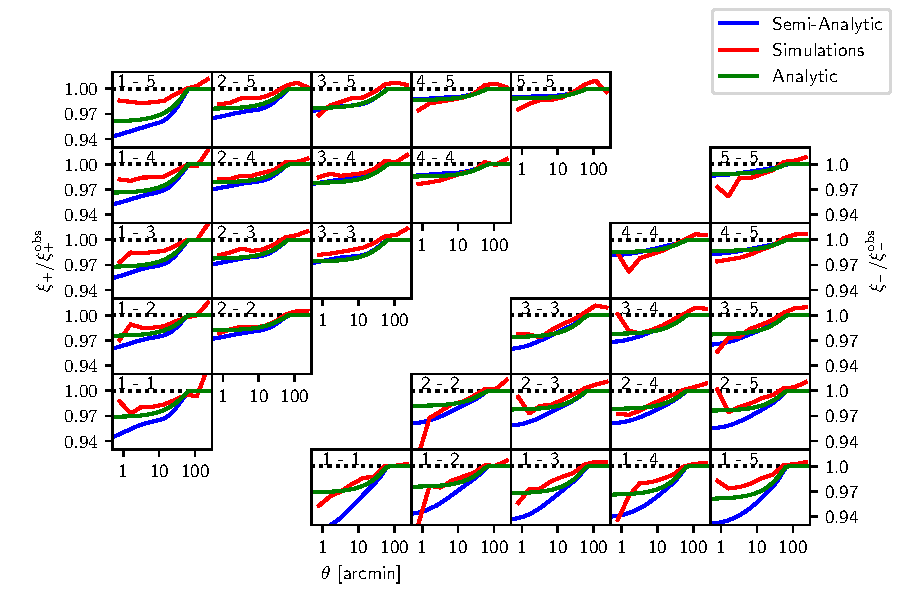
\includegraphics[width=1\textwidth]{allxis_0111.pdf}
	\caption[The ratio of modelled to observed correlation functions]{The ratio of modelled to observed correlation functions for the analytic method (green), the semi-analytic method (blue) and the numerical simulations (red) for a cross-correlation of all redshift bins. The upper left triangle shows the ratios for $\xi_+$, the lower right triangle the ones for $\xi_-$. The numbers in the plots denote the respective bins.}
	\label{fig:all_xis}
	\end{figure}
	
In Figure \ref{fig:all_xis} we can see a plot of the ratios between the modelled and observed correlation functions for each of the three methods. It is interesting to note that for the higher redshift bins, the analytic and semi-analytic methods seem to agree on the whole range of $\theta$. However, especially for $\xi_-$, the lower redshift bins show a significant discrepancy between those two methods, which is expected: The power-law $
\la |\gamma|\ra \propto z^{0.85}
$
inspired by \citet{2006APh....26...91V} is redshift-dependent and thus not valid for all tomographic bins. Furthermore, especially the lower tomographic bins experience a strong variation in average redshift, whereas the simple model is only valid for small variations in redshift.

We also observe that in the semi-analytic model, $\xi_-$ seems to be much stronger affected by this effect. We can explain this by investigating Figure \ref{fig:bessel}: Following Equation \eqref{eq:xipm_from_pkappa}, $\xi_+$ is computed by filtering the power spectrum with the 0-th order Bessel function. This function peaks at $\ell\theta=0$, meaning that for all values of $\theta$, the correlation function $\xi_+$ is sensitive to small values of $\ell$, corresponding to large separations $\theta$. However, $\xi_-$ is obtained by filtering with the 4-th order Bessel function, which peaks at approximately $\ell\theta\approx 5$, so for different $\theta$ this function is sensitive to varying parts of the convergence power spectrum. A more detailed analysis of this can be found in the Appendix of \citet{2017MNRAS.471.4412K}.

The simulations seem to be in rough agreement with the models, but there are some significant differences. After a thorough analysis we explain these discrepancies the following way: The simulations were performed on a $100\,\rm{deg}^2$ field, which means that shot-noise of the fields plays a significant role. After performing the same simulations for a different distribution of depth between the pointings and obtaining completely different results, we are quite certain that this is the dominating effect. The implications of this and possible mitigation strategies will be discussed in Chapter \ref{sec:discussion}.

To estimate the effects on the cosmological parameters, we performed a Markov-Chain-Monte-Carlo (MCMC) simulation. Given a fiducial cosmology, we calculated a reference set of correlation functions and divided them by the ratios plotted in Figure \ref{fig:all_xis}, to simulate an observed correlation function. We then calculated sets of correlation functions for different cosmologies and computed the difference to the reference functions, weighted by the respective elements in the inverse covariance matrix $C\inv$ of the correlation functions, which was determined by \citet{2018arXiv181206076H}. The code for this method is a modified version of work by Jan Luca van den Busch.

As our main interest is the investigation of the parameter $S_8$, we chose to limit our analysis to the $\Omega_{\rm m} - \sigma_8$ plane. For the KV450 survey we saw a slight change in the results for $\Omega_{\rm m}$ and $\sigma_8$, but it was far from being relevant. To estimate the impact for the upcoming Euclid-survey we divided the covariance matrix $C$ by 30, to account for the increased survey area\footnote{We want to stress that this is in no way a valid forecast for the Euclid survey. However, we are positive that the qualitative question whether this effect will be relevant, can be answered using this method.}. In these simulations we saw a bias of about $1\sigma$ both for $\Omega_{\rm m}$ and $\sigma_8$. Curiously, both parameters changed in a way such that the parameter $S_8$ stayed unbiased. The exact values determined by the MCMC simulations can be found in Table \ref{tab:parameter_constraints}, the likelihood functions can be found in Figures \ref{fig:mcmc_kids} and \ref{fig:mcmc_euclid} in the Appendix.
{
\renewcommand{\arraystretch}{1.3}
\begin{table}
\centering
\caption[Parameter constraints from the MCMC simulations]{Parameter constraints from the MCMC simulations for a KiDS-like and a `Euclid-like' survey subject to varying depth.}
\begin{tabular}{c | S S S }
\centering
 & {$\Omega_{\rm m}$} & {$\sigma_8$} & {$S_8$} \\
 \toprule
 Fiducial & 0.250 & 0.849 & 0.775 \\
 KiDS-like & 0.290$_{-0.091}^{+0.045}$ & 0.80\phantom{0}$_{-0.14}^{+0.14}$ & 0.763\phantom{9}$_{-0.027}^{+0.044}$ \\
 `Euclid-like' & 0.264$_{-0.013}^{+0.011}$ & 0.828$_{-0.025}^{+0.025}$ & 0.7759$_{-0.0059}^{+0.0067}$
\end{tabular}
\label{tab:parameter_constraints}
\end{table}
}

As the next step we wanted to investigate the B-modes created by this effect. For this we decided to use the COSEBIs discussed in Section \ref{sec:e_and_bmode_separation}. As the COSEBIs separate E- and B-modes based on a finite interval $[\theta_{\rm{min}},\theta_{\rm{max}}]$, they are convenient to use for real data. As varying depth modifies the correlation functions on scales from $0\arcmin$ to roughly $85\arcmin$, we chose our interval as $\theta_{\rm{min}}=0.\!^\prime 5$ and $\theta_{\rm{max}}=100\arcmin$ to be especially sensitive to this effect. We calculated the logarithmic COSEBIs \citep[compare][]{2010A&A...520A.116S} for a reference set of correlation functions $\xi_\pm$ and a set of correlation functions simulating the observed ones, $\xi_\pm\obs$. To minimize numerical errors, we determined both correlation functions in $10^6$ angular bins. The E- and B-modes determined by this analysis can be seen in Figure \ref{fig:cosebis_all}. As the reference correlation functions should not show any B-modes, they serve as an estimate for the numerical errors. As one can see, those errors are several orders of magnitude lower than the determined E- and B-modes for low $n$, but they rise with increasing $n$. This is not surprising, as for higher $n$ the filter functions $T_{\pm,n}$ from Equation \eqref{eq:ebmodes1} oscillate faster and are thus more prone to numerical errors. As \citet{2018arXiv181002353A} pointed out, $\xi_\pm$ are relatively smooth functions and are thus already pretty well constrained by the first few E-modes. This is the reason why the E-modes start to rapidly drop for higher $n$. The B-modes, however, can have more complicated origins, so that they do not necessarily drop as quickly for higher modes. Due to that, for high $n$ the B-modes actually surpass the E-modes.
\begin{figure}
\centering
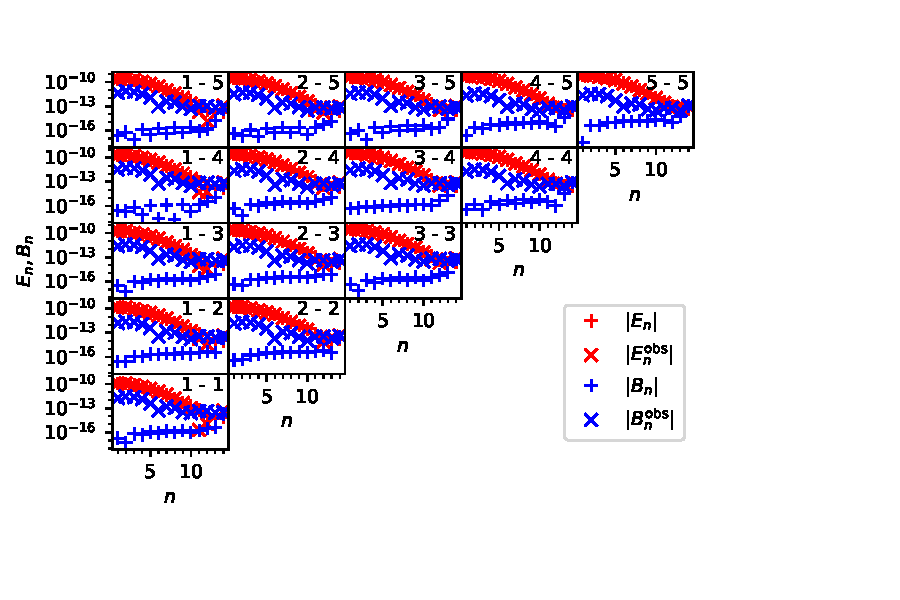
\includegraphics[trim={0cm 1cm 2.5cm 0.5cm},clip,width = 0.9\textwidth]{cosebis_all.pdf}
\caption[E- and B-modes of the reference and the observed correlation functions]{Logarithmic E- and B-modes of the reference and the observed correlation functions for an angular range of $\theta_{\rm{min}}=0.\!^\prime 5,\,\theta_{\rm{max}}=100\arcmin$.}
\label{fig:cosebis_all}
\end{figure}

When we focus on the difference between reference and observed modes (depicted in Figure \ref{fig:cosebis_eandb}), we notice that the difference in E-modes is roughly as high as the one in the B-modes (where the B-modes of the reference function are zero). We also notice that both the E-modes and the B-modes show a characteristic pattern that is consistent throughout all redshift bins.

\begin{figure}
\centering
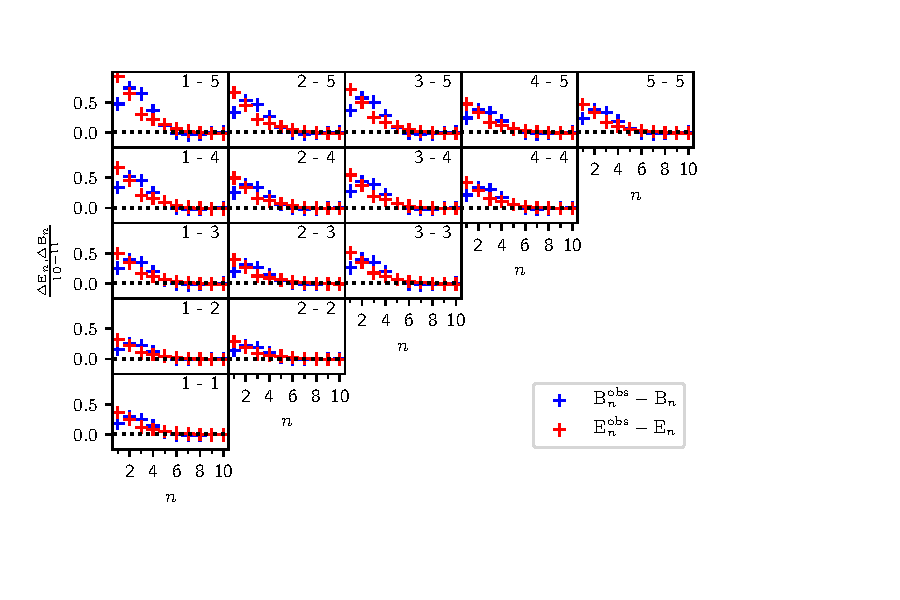
\includegraphics[trim={0cm 1cm 2.5cm 0.5cm},clip,width = 0.9\textwidth]{eandbmodes0p5t100.pdf}
\caption[Difference in E- and B-modes between the reference and the observed correlation functions]{Difference in the logarithmic E- and B-modes between the reference and the observed correlation functions for an angular range of $\theta_{\rm{min}}=0.\!^\prime 5,\,\theta_{\rm{max}}=100\arcmin$.}
\label{fig:cosebis_eandb}
\end{figure}


%%% Local Variables: 
%%% mode: latex
%%% TeX-master: "../mythesis"
%%% End: 